
\section{The correctness of distributed algorithms}
Distributed algorithms run on multiple processors without centralized control and are central to both everyday devices (e.g., smartphones) and safety-critical systems (e.g., medical devices, trains, aircraft, spacecraft).
Errors in distributed algorithms can have severe consequences, such as the loss of critical data or even human life. Ensuring their correctness is vital but challenging due to the inherent complexity of these systems~\cite{heiser2010theroad, lamport2019thebyzantine}. 
The Needham-Schroeder protocol~\cite{needham1978using}\textemdash intended for two computers to verify each other's identity\textemdash exemplifies this challenge: a serious security flaw was discovered 17 years after it publication~\cite{lowe1996breaking}.
To address the challenge of uncovering subtle vulnerabilities in distributed algorithms, one natural approach is to test all possible scenarios. This is effective when the number of scenarios is small, but becomes infeasible otherwise. For example, when there are infinitely many scenarios, program testing may reveal bugs, but cannot prove the absence of bugs\textemdash a fundamental limitation that motivates the use of formal verification techniques.

Formal verification techniques are mathematically rigorous methods for proving system correctness. 
This thesis focuses on automated verification techniques~\cite{clarke2018model, contejean2011automated, cortier2014formal, urbain2004modular,steinbach1995simplification,kassing2024dependency,marche2004modular} for specific properties, which perform proof search automatically and need little user intervention.
   
\section{Automated verification techniques}
Automated verification techniques are particularly interesting because they can be implemented as automated tools accessible to non-experts in formal verification while also accelerating verification for experts.
To verify a specific property of an algorithm, the user needs only to model the algorithm in a required formalism, and the tool then automatically checks conditions that mathematically imply the target property. To further ensure the correctness of results, advanced tools generate certificates verifiable by proof assistants~\cite{contejean2011automated}. 
Although theoretically incomplete for certain properties (meaning some inputs may yield no answer), well-designed techniques can handle many practical cases and significantly reduce verification effort. 
To enable such methods, distributed algorithms must be modeled using a formalism that facilitates rigorous analysis of their properties. Specifically, states and behaviors of distributed algorithms must be formally represented.

\section{Finite edge-labeled directed multigraphs} 
Finite edge-labeled directed multigraphs provide an intuitive yet formal way to model states of distributed algorithms: Computational units are represented by nodes; communication channels are represented by edges; states of the system are modeled by graphs whose edges have labels representing information encoded in computational units and states of communication channels. 

For example, consider the graph $\mathcal{G}$ shown in the following Figure~\ref{fig:graph_modeling_state_network}, enclosed in a box labeled with its name in the top-left corner. 
The graph models a distributed network of six computational units.
Each node represents a computational unit; a node's state is indicated by the label of its self-loop; each edge represents a communication channel. In Figure~\ref{fig:graph_modeling_state_network}, node $1$ labeled by $A$ represents an active computational unit, the other nodes labeled by $N$ represent neutral computational units, and edges labeled by $0$ represent communication channels in state $0$. \todo{links on number only}
\begin{figure}[H]
        \centering
        \resizebox{0.4\textwidth}{!}{
                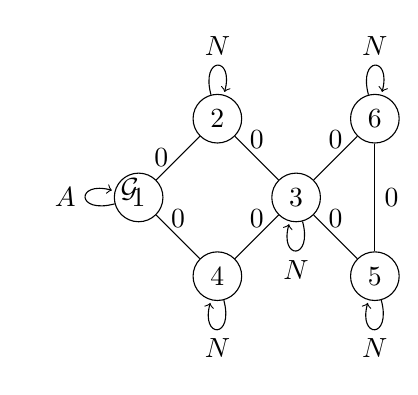
\begin{tikzpicture}
                    \graphbox{\( \mathcal{G} \)}{0mm}{0mm}{50mm}{50mm}{-10mm}{-25mm}{
                        \node[draw, circle] (n1) at (0,0) {$1$};
                        \node[draw, circle] (n2) at (1,1) {$2$};
                        \node[draw, circle] (n4) at (1,-1) {$4$};
                        \node[draw, circle] (n3) at (2,0) {$3$}; 
                        \node[draw, circle] (n5) at (3,-1){$5$};
                        \node[draw, circle] (n6) at (3,1){$6$};
                        \draw[-] (n1) edge node[left] {$0$} (n2);
                        \draw[-] (n2) edge node[above] {$0$} (n3);
                        \draw[-] (n3) edge node[above] {$0$} (n4);
                        \draw[-] (n4) edge node[above] {$0$} (n1);
                        \draw[-] (n3) edge node[above] {$0$} (n6);
                        \draw[-] (n6) edge node[right] {$0$} (n5);
                        \draw[-] (n5) edge node[above] {$0$} (n3);  
                        \draw[->] (n1) edge [loop left] node {$A$} (n1);
                        \draw[->] (n2) edge [loop above] node {$N$} (n2);
                        \draw[->] (n3) edge [loop below] node {$N$} (n3);
                        \draw[->] (n4) edge [loop below] node {$N$} (n4);
                        \draw[->] (n5) edge [loop below] node {$N$} (n5);
                        \draw[->] (n6) edge [loop above] node {$N$} (n6);
                    } 
                \end{tikzpicture} 
    }
    \caption{A graph modeling a network configuration. An undirected edge between nodes $u$ and $v$ denotes two directed edges from $u$ to $v$ and from $v$ to $u$. The numbers inside the nodes are node identifiers.}
    \label{fig:graph_modeling_state_network}
\end{figure}

\section{Graph transformation}
Graph transformation provides an intuitive yet formal way to model algorithm behaviors: state changes are modeled by replacing subgraphs of a graph with other subgraphs according to transformation rules.

As an example, consider a distributed spanning-tree construction algorithm on a connected network, where one computational unit is active, all other nodes are neutral, and every channel is initially in state $0$. An example initial configuration is shown in Figure~\ref{fig:graph_modeling_state_network}. 
The algorithm operates as follows: when an active unit detects a neutral neighbor via a channel in state $0$, it activates the neighbor and updates the channel to state $1$.
 This behavior is captured by the graph transformation rule in the following Figure~\ref{fig:intro:graph_transformation_rule_0}.
 \begin{figure}[H]
        \centering 
            \resizebox{0.48\textwidth}{!}{
        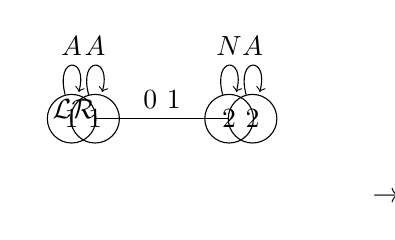
\begin{tikzpicture}
                    \graphbox{\( \mathcal{L} \)}{0mm}{0mm}{34mm}{20mm}{-8mm}{-15mm}{
                        \node[draw, circle] (x) at (0,0) {$1$};  
                        \node[draw, circle] (y) at (2,0) {$2$};
                        \draw[-] (x) -- node[midway,above] {$0$} (y) ;
                                    \draw[->] (x) edge [loop above] node {$A$} (x);
                        \draw[->] (y) edge [loop above] node {$N$} (y);
                    }
                    \graphbox{\( \mathcal{R} \)}{40mm}{0mm}{34mm}{20mm}{-8mm}{-15mm}{
                        \node[draw, circle]  (x) at (0,0) {$1$};  
                        \node[draw, circle]  (y) at (2,0) {$2$};
                        \draw[-] (x) -- node[midway,above] {$1$} (y) ;
                        \draw[->] (x) edge [loop above] node {$A$} (x);
                        \draw[->] (y) edge [loop above] node {$A$} (y);
                    }  
                    \node () at (37mm,-10mm) {\( \rightarrow \)}; % K -> L
        \end{tikzpicture}
            }
        \caption{Graph rewriting rule for the spanning-tree construction of a connected network with one node labeled by $A$ and all other nodes labeled by $N$ and all edges labeled by $0$. It relabels an occurrence of \(\mathcal{L}\) to \(\mathcal{R}\).}
        \label{fig:intro:graph_transformation_rule_0}
    \end{figure}
\noindent This rule applies as follows: when an active unit detects a neutral neighbor via a channel in state $0$, the corresponding subgraph \(\mathcal{L}\) appears in the network model and is replaced by the subgraph \(\mathcal{R}\), which represents the neighbor's activation and the channel updated to state $1$.

Given an initial finite edge-labeled directed multigraph in which all edges are labeled \textit{0} and all nodes are in the neutral state $N$ except for a single node in the active state $A$, the subgraph induced by edges labeled \textit{1} constitutes a spanning tree once no further rule applications are possible. A sample execution sequence starting from the initial configuration, previously defined and illustrated in Figure~\ref{fig:graph_modeling_state_network}, is shown in Figure~\ref{fig:intro_sequence_of_transformation}, where self-loops are omitted and their labels are displayed directly on the nodes to improve readability. 
% When no further rule applications are possible, the subgraph induced by edges labeled $1$ constitutes a spanning tree (see rightmost and bottom most graphs in Figure~\ref{fig:intro_sequence_of_transformation}).

    \begin{figure}[H]
        \centering
        \resizebox{0.28\textwidth}{!}{
                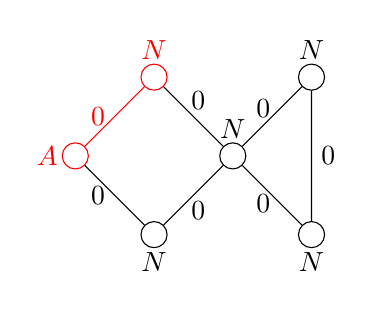
\begin{tikzpicture}
                    \node[draw, red,circle] (n1) at (0,0) {};
                    \node[draw, red,circle] (n2) at (1,1) {};
                    \node[draw, circle] (n4) at (1,-1) {};
                    \node[draw, circle] (n3) at (2,0) {};
                    \node[draw, circle] (n5) at (3,-1){};
                    \node[draw, circle] (n6) at (3,1){};
                    \draw[-,red] (n1)--(n2);
                    \draw[-] (n2)--(n3)--(n4);
                    \draw[-] (n4)--(n1);
                    \draw[-] (n3)--(n6)--(n5)--(n3);
                    \draw[transparent, rounded corners,rotate around={45:(0,-0.5)}, dotted] (0,-0.5) rectangle (2.2,0.3) ;
                    \draw[transparent, rounded corners,rotate around={-45:(0,0.5)}, dotted] (0,0.5) rectangle (2.2,-0.3) ;   

                    \draw(-0.1,0) node[left] {\textcolor{red}{$A$}};
                    \draw(1,1.1) node[above] {\textcolor{red}{$N$}};
                    \draw(1,-1.1) node[below] {$N$};
                    \draw(2,0.1) node[above] {$N$};
                    \draw(3,1.1) node[above] {$N$};
                    \draw(3,-1.1) node[below] {$N$};

                    % edge labels
                    \draw(1.35,0.7) node[right] {$0$};
                    \draw(1.35,-0.7) node[right] {$0$};
                    \draw(0.5,0.5) node[left] {\textcolor{red}{$0$}};
                    \draw(0.5,-0.5) node[left] {$0$};
                    \draw(2.6,0.6) node[left] {$0$};
                    \draw(2.6,-0.6) node[left] {$0$};
                    \draw(3,0) node[right] {$0$};
                \end{tikzpicture}
    }
  \resizebox{0.28\textwidth}{!}{
                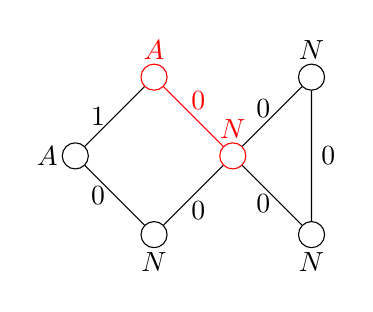
\begin{tikzpicture}
                    \node[draw, circle] (n1) at (0,0) {};
                    \node[draw, red,circle] (n2) at (1,1) {};
                    \node[draw, circle] (n4) at (1,-1) {};
                    \node[draw, red,circle] (n3) at (2,0) {};
                    
                    \node[draw, circle] (n5) at (3,-1){};
                    \node[draw, circle] (n6) at (3,1){};
        
                    \draw[-] (n1)--(n2);
                    \draw[-,red] (n2)--(n3);
                    \draw[-] (n3)--(n4);
                    \draw[-] (n4)--(n1);
                    \draw[-] (n3)--(n6)--(n5)--(n3);
        
                    \draw[transparent, rounded corners,rotate around={45:(0,-0.5)}, dotted] (0,-0.5) rectangle (2.2,0.3) ;
                    \draw[transparent, rounded corners,rotate around={-45:(0,0.5)}, dotted] (0,0.5) rectangle (2.2,-0.3) ;
    
                    \draw(-0.1,0) node[left] {$A$};
                    \draw(1,1.1) node[above] {\textcolor{red}{$A$}};
                    \draw(1,-1.1) node[below] {$N$};
                    \draw(2,0.1) node[above] {\textcolor{red}{$N$}};
                    \draw(3,1.1) node[above] {$N$};
                    \draw(3,-1.1) node[below] {$N$};

                    % edge labels
                    \draw(1.35,0.7) node[right] {\textcolor{red}{$0$}};
                    \draw(1.35,-0.7) node[right] {$0$};
                    \draw(0.5,0.5) node[left] {$1$};
                    \draw(0.5,-0.5) node[left] {$0$};
                    \draw(2.6,0.6) node[left] {$0$};
                    \draw(2.6,-0.6) node[left] {$0$};
                    \draw(3,0) node[right] {$0$};
                \end{tikzpicture}
}
\resizebox{0.28\textwidth}{!}{
                    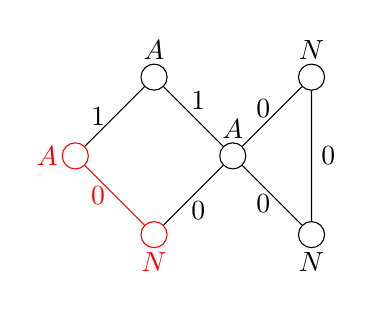
\begin{tikzpicture}
                        \node[draw, red,circle] (n1) at (0,0) {};
                        \node[draw, circle] (n2) at (1,1) {};
                        \node[draw, red,circle] (n4) at (1,-1) {};
                        \node[draw, circle] (n3) at (2,0) {};
                        
                        \node[draw, circle] (n5) at (3,-1){};
                        \node[draw, circle] (n6) at (3,1){};
            
                    \draw[-] (n1)--(n2);
                    \draw[-] (n2)--(n3);
                    \draw[-] (n3)--(n4);
                    \draw[-,red] (n4)--(n1);
                    \draw[-] (n3)--(n6)--(n5)--(n3);
            
                        \draw[transparent, rounded corners,rotate around={45:(0,-0.5)}, dotted] (0,-0.5) rectangle (2.2,0.3) ;
                        \draw[transparent, rounded corners,rotate around={-45:(0,0.5)}, dotted] (0,0.5) rectangle (2.2,-0.3) ;
    
                        \draw(-0.1,0) node[left] {\textcolor{red}{$A$}};
                        \draw(1,1.1) node[above] {$A$};
                        \draw(1,-1.1) node[below] {\textcolor{red}{$N$}};
                        \draw(2,0.1) node[above] {$A$};
                        \draw(3,1.1) node[above] {$N$};
                        \draw(3,-1.1) node[below] {$N$};
    
                        % edge labels
                        \draw(1.35,0.7) node[right] {$1$};
                        \draw(1.35,-0.7) node[right] {$0$};
                        \draw(0.5,0.5) node[left] {$1$};
                        \draw(0.5,-0.5) node[left] {\textcolor{red}{$0$}};
                        \draw(2.6,0.6) node[left] {$0$};
                        \draw(2.6,-0.6) node[left] {$0$};
                        \draw(3,0) node[right] {$0$};
                    \end{tikzpicture}
}


\resizebox{0.28\textwidth}{!}{
                    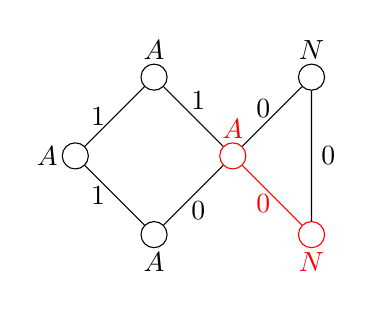
\begin{tikzpicture}
                        \node[draw, circle] (n1) at (0,0) {};
                        \node[draw, circle] (n2) at (1,1) {};
                        \node[draw, circle] (n4) at (1,-1) {};
                        \node[draw, red,circle] (n3) at (2,0) {};
                        
                        \node[draw, red,circle] (n5) at (3,-1){};
                        \node[draw, circle] (n6) at (3,1){};
            
                        \draw[-] (n1)--(n2);
                        \draw[-] (n2)--(n3);
                        \draw[-] (n3)--(n4);
                        \draw[-] (n4)--(n1);
                        \draw[-] (n3)--(n6)--(n5);
                        \draw[-,red] (n5)--(n3);
            
                        \draw[transparent, rounded corners,rotate around={45:(0,-0.5)}, dotted] (0,-0.5) rectangle (2.2,0.3) ;
                        \draw[transparent, rounded corners,rotate around={-45:(0,0.5)}, dotted] (0,0.5) rectangle (2.2,-0.3) ;

                        \draw(-0.1,0) node[left] {$A$};
                        \draw(1,1.1) node[above] {$A$};
                        \draw(1,-1.1) node[below] {$A$};
                        \draw(2,0.1) node[above] {\textcolor{red}{$A$}};
                        \draw(3,1.1) node[above] {$N$};
                        \draw(3,-1.1) node[below] {\textcolor{red}{$N$}};
    
                        % edge labels
                        \draw(1.35,0.7) node[right] {$1$};
                        \draw(1.35,-0.7) node[right] {$0$};
                        \draw(0.5,0.5) node[left] {$1$};
                        \draw(0.5,-0.5) node[left] {$1$};
                        \draw(2.6,0.6) node[left] {$0$};
                        \draw(2.6,-0.6) node[left] {\textcolor{red}{$0$}};
                        \draw(3,0) node[right] {$0$};
                    \end{tikzpicture}
}
\resizebox{0.28\textwidth}{!}{
                    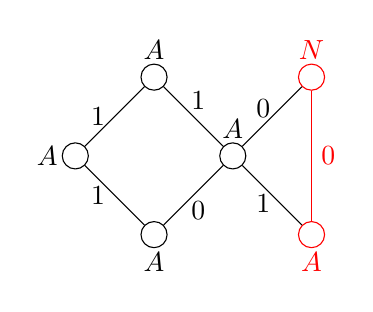
\begin{tikzpicture}
                        \node[draw, circle] (n1) at (0,0) {};
                        \node[draw, circle] (n2) at (1,1) {};
                        \node[draw, circle] (n4) at (1,-1) {};
                        \node[draw,circle] (n3) at (2,0) {};
                        
                        \node[draw, red,circle] (n5) at (3,-1){};
                        \node[draw, red,circle] (n6) at (3,1){};
            
                        \draw[-] (n1)--(n2)--(n3)--(n4);
                        \draw[-] (n4)--(n1);
                        \draw[-] (n3)--(n6);
                        \draw[-,red] (n6)--(n5);
                        \draw[-] (n5)--(n3);
            
                        \draw[transparent, rounded corners,rotate around={45:(0,-0.5)}, dotted] (0,-0.5) rectangle (2.2,0.3) ;
                        \draw[transparent, rounded corners,rotate around={-45:(0,0.5)}, dotted] (0,0.5) rectangle (2.2,-0.3) ;
              
                        \draw(-0.1,0) node[left] {$A$};
                        \draw(1,1.1) node[above] {$A$};
                        \draw(1,-1.1) node[below] {$A$};
                        \draw(2,0.1) node[above] {$A$};
                        \draw(3,1.1) node[above] {\textcolor{red}{$N$}};
                        \draw(3,-1.1) node[below] {\textcolor{red}{$A$}};

                        % edge labels
                        \draw(1.35,0.7) node[right] {$1$};
                        \draw(1.35,-0.7) node[right] {$0$};
                        \draw(0.5,0.5) node[left] {$1$};
                        \draw(0.5,-0.5) node[left] {$1$};
                        \draw(2.6,0.6) node[left] {$0$};
                        \draw(2.6,-0.6) node[left] {$1$};
                        \draw(3,0) node[right] {\textcolor{red}{$0$}};
                    \end{tikzpicture}
}
\resizebox{0.28\textwidth}{!}{
                    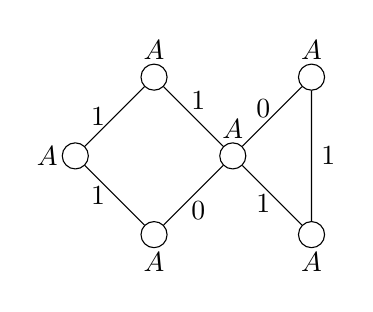
\begin{tikzpicture}
                        \node[draw, circle] (n1) at (0,0) {};
                        \node[draw, circle] (n2) at (1,1) {};
                        \node[draw, circle] (n4) at (1,-1) {};
                        \node[draw, circle] (n3) at (2,0) {};
                        
                        \node[draw, circle] (n5) at (3,-1){};
                        \node[draw, circle] (n6) at (3,1){};
            
                        \draw[-] (n1)--(n2)--(n3)--(n4);
                        \draw[-] (n4)--(n1);
                        \draw[-] (n3)--(n6)--(n5)--(n3);
            
                        \draw[transparent, rounded corners,rotate around={45:(0,-0.5)}, dotted] (0,-0.5) rectangle (2.2,0.3) ;
                        \draw[transparent, rounded corners,rotate around={-45:(0,0.5)}, dotted] (0,0.5) rectangle (2.2,-0.3) ;
                        \draw(-0.1,0) node[left] {$A$};
                        \draw(1,1.1) node[above] {$A$};
                        \draw(1,-1.1) node[below] {$A$};
                        \draw(2,0.1) node[above] {$A$};
                        \draw(3,1.1) node[above] {$A$};
                        \draw(3,-1.1) node[below] {$A$};
     
                        % edge labels
                        \draw(1.35,0.7) node[right] {$1$};
                        \draw(1.35,-0.7) node[right] {$0$};
                        \draw(0.5,0.5) node[left] {$1$};
                        \draw(0.5,-0.5) node[left] {$1$};
                        \draw(2.6,0.6) node[left] {$0$};
                        \draw(2.6,-0.6) node[left] {$1$};
                        \draw(3,0) node[right] {$1$};
                    \end{tikzpicture}
}
        \caption{Sequence of graph transformation, to be read from left to right and from top to bottom. At each graph, the subgraph in red is to be relabeled according to the rule to obtain the next graph.}
        \label{fig:intro_sequence_of_transformation}
    \end{figure}
 
 Graph transformation has many applications, such as topology-based geometric modeling~\cite{poudret2007topology,poudret2008graph_transformation, belhaouari2014jerboa, bellet2017geometric, pascale2022Geometric_modeling,arnould2022preserving_consistency}, DNA computing~\cite{harju2004tutorial_dna_computation}, life sciences~\cite{behr2021rewriting_life_sciences}, programming~\cite{plump2009graph_programming_language}, administrative access control policies~\cite{bertolissi2025category_based, bertolissi2021graph_based,koch2001specification_evolution_access_control},and software engineering and security~\cite{heckel2020software_engineers}. Its broad applicability stems from the fact that graphs and graph-like structures provide a natural and intuitive way to model complex systems. 
 
 A predominant school of thought in this area is called algebraic graph rewriting~\cite{ehrig1997handbook1,ehrig1999handbook2,ehrig1999handbook3}, which uses concepts from category theory~\cite{pierce1991basic,barr1990category,maclane2013categories} to define graph transformation. 
 There are different notions of graphs in the literature for different applications, such as edge-labeled multigraphs~\cite{konig2018atutorial,corradini1997algebraic}, hypergraphs~\cite{plump1993hypergraph}, attributed graphs~\cite{ehrig2006fundamentals}, and polygraphs~\cite{ara2023polygraphs}.
 The language of category theory abstracts away from the details of the different notions of graphs, provided that the notion of graph satisfies certain properties~\cite{lack2004adhesive,overbeek2023graph}.  
This enables a uniform definition of graph transformation, and leads to an elegant definition of graph transformation. 

 Double-pushout (DPO) graph rewriting~\cite{corradini1997algebraic,habel2001double} is among the most studied algebraic graph transformation. A DPO graph rewriting rule consists of two functions that preserve graph structure, namely $l:\mathcal{K} \to \mathcal{L}$ and $r:\mathcal{K} \to \mathcal{R}$,
 Here, \(\mathcal{L}\) is the left-hand side graph encoding the rule's preconditions, \(\mathcal{R}\) is the right-hand side graph describing the postconditions, and \(\mathcal{K}\) is the interface graph—the part common to \(\mathcal{L}\) and \(\mathcal{R}\) that is preserved by the rule and serves as the interface to the surrounding context. A DPO graph rewriting rule is commonly denoted by \(\mathcal{L} \xleftarrow{l} \mathcal{K} \xrightarrow{r} \mathcal{R}\) in the literature.
 
 As an example, the graph transformation rule, previously defined and illustrated in Figure~\ref{fig:intro:graph_transformation_rule_0}, can be represented as the DPO graph rewriting rule shown in Figure~\ref{fig:intro:graph_transformation_rule_0_dpo}.

%  \begin{center}
 \begin{figure}[H]
    \centering
    \resizebox{0.85\textwidth}{!}{
       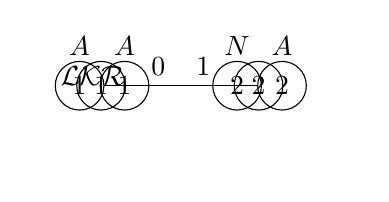
\begin{tikzpicture} 
                    \graphbox{\( \mathcal{L} \)}{-40mm}{-3mm}{34mm}{15mm}{-8mm}{-9mm}{
                        \node[draw, circle] (x) at (0,0) {$1$};  
                        \node[draw, circle] (y) at (2,0) {$2$};
                        \draw[-] (x) -- node[midway,above] {$0$} (y) ;
                        \node  () at (0,0.5) {$A$};  
                        \node () at (2,0.5) {$N$};
                    } 
                    \graphbox{\( \mathcal{K} \)}{0mm}{-3mm}{34mm}{15mm}{-8mm}{-9mm}{
                        \node[draw, circle] (x) at (0,0) {$1$};  
                        \node[draw, circle] (y) at (2,0) {$2$};
                    } 
                    \graphbox{\( \mathcal{R} \)}{40mm}{-3mm}{34mm}{15mm}{-8mm}{-9mm}{
                        \node[draw, circle] (x) at (0,0) {$1$};  
                        \node[draw, circle] (y) at (2,0) {$2$};
                        \draw[-] (x) -- node[midway,above] {1} (y) ;
                        \node  () at (0,0.5) {$A$};  
                        \node () at (2,0.5) {$A$};
                    }  
                    \node () at (37mm,-10mm) {\( \rightarrowtail \)}; % K -> L
                    \node () at (-3mm,-10mm) {\( \leftarrowtail  \)}; % K -> L
                \end{tikzpicture}
    }
            % \end{center}
    \caption{A DPO graph rewriting rule which replaces an occurrence of \(\mathcal{L}\) by an occurrence of \(\mathcal{R}\).
    % while preserving the two extremal nodes.
    }
    \label{fig:intro:graph_transformation_rule_0_dpo}
    \end{figure} 

To apply a DPO graph rewriting rule $\mathcal{L} \overset{l}{\leftarrow} \mathcal{K} \overset{r}{\rightarrow} \mathcal{R}$ to a host graph $\mathcal{G}$, one must first identify an occurrence of $\mathcal{L}$ in which a subgraph is designed as the interface graph. The other elements of the host graph $\mathcal{G}$ together with the interface graph form the context graph $\mathcal{C}$ of the rewriting step.
The graph $\mathcal{G}$ is thus decomposed into the occurrence of $\mathcal{L}$ and $\mathcal{C}$. 
Then, one modifies the occurrence of $\mathcal{L}$ (by removing some nodes and edges and adding some fresh nodes and edges while keeping the interface graph unchanged, and identifying nodes in the interface graph)
to obtain an occurrence of $\mathcal{R}$. Finally, the result graph is obtained by gluing the occurrence of $\mathcal{R}$ with $\mathcal{C}$ via the interface graph $\mathcal{K}$.
As an example, 
consider the graph transformation rule, shown in the following Figure~\ref{fig:intro:graph_transformation_rule_dpo_sssssfggaaadww}.
  \begin{figure}[H]
    \centering
% \begin{center} 
    \resizebox{0.85\textwidth}{!}{
    \begin{tikzpicture}
                    \graphbox{\( \mathcal{L} \)}{-40mm}{-3mm}{34mm}{15mm}{2mm}{2mm}{
                        \coordinate (o) at (0mm,-11mm); 
                        \node[draw,circle] (l1) at ($(o)+(-10mm,0mm)$) {$1$};
                        \node[draw,circle] (l2) at ($(l1)+(2,0)$) {$2$};
                        \node[draw,circle] (l3) at ($(l1) + (1,0)$) {$3$};
                        \draw (l1) -- (l3) node[midway,above] {$a$};
                        \draw (l3) -- (l2) node[midway,above] {$a$};
                    } 
                    \graphbox{\( \mathcal{K} \)}{0mm}{-3mm}{34mm}{15mm}{2mm}{2mm}{
                        \coordinate (o) at (0mm,-11mm); 
                        \node[draw,circle] (l1) at ($(o)+(-10mm,0mm)$) {$1$};
                        \node[draw,circle] (l2) at ($(l1)+(2,0)$) {$2$};
                    } 
                    \graphbox{\( \mathcal{R} \)}{40mm}{-3mm}{34mm}{15mm}{2mm}{2mm}{
                        \coordinate (o) at (0mm,-11mm); 
                        \node[draw,circle] (l1) at ($(o)+(-10mm,0mm)$) {$1$};
                        \node[draw,circle] (l2) at ($(l1)+(2,0)$) {$2$};
                    }  
                    \node () at (37mm,-10mm) {\( \overset{l}{\longrightarrow}\)}; % K -> L
                    \node () at (-3mm,-10mm) {\( \overset{r}{\longleftarrow}  \)}; % K -> L
                \end{tikzpicture}
    }
            % \end{center}
    \caption{A DPO graph rewriting rule which removes the middle node and edges of an occurrence of $\mathcal{L}$.}
    \label{fig:intro:graph_transformation_rule_dpo_sssssfggaaadww}
\end{figure}
\noindent The graph $\mathcal{G}$ shown in Figure~\ref{fig:intro:graph_G} can be rewritten to yield the graph $\mathcal{H}$ shown in Figure~\ref{fig:intro:graph_H} by applying the following DPO graph rewriting rule, defined earlier,
% in Figure~\ref{fig:intro:graph_transformation_rule_dpo} 
to the unique occurrence 
\raisebox{2pt}{
            \scalebox{0.7}{\tikz[baseline=-0.5ex]{
            \node [draw,circle] (z) at (-1,0) {1};
            \node [draw,circle] (x) at (0,0) {3};
            \node[draw,circle] (y) at (1,0) {2};
            \draw (z)--(x) node[midway, above] {$a$};
            \draw (x)--(y) node[midway, above] {$a$};
        }}}
of $\mathcal{L}$ in $\mathcal{G}$.
Specifically, in this occurrence the subgraph matched to the interface graph $\mathcal{K}$ is the subgraph shown in black in Figure~\ref{fig:intro:decomposition_of_G}; the graph $\mathcal{G}$ is decomposed, as shown in Figure~\ref{fig:intro:decomposition_of_G}, into the occurrence of $\mathcal{L}$ (elements shown in orange and black) and the context graph $\mathcal{C}$ (elements shown in blue and black) gluing via the interface graph (elements shown in black).
%  The interface graph is the subgraph shown in black in Figure~\ref{fig:intro:decomposition_of_G}. 
 The rule removes the orange part of the occurrence of $\mathcal{L}$ to obtain an occurrence of $\mathcal{R}$. 
The result graph $\mathcal{H}$ is obtained by gluing the occurrence of $\mathcal{R}$ and the context graph $\mathcal{C}$ via the interface graph.
\begin{figure}[H]
    \centering
    \begin{subfigure}{0.4\textwidth}
        \centering
        \begin{tikzpicture}
            \graphbox{\( \mathcal{G} \)}{0mm}{-22mm}{34mm}{22mm}{2mm}{-3mm}{
                    \coordinate (o) at (0mm,-3mm); 
                    \node[draw,circle] (l1) at ($(o)+(-10mm,0mm)$) {$1$};
                    \node[draw,circle] (l2) at ($(l1)+(2,0)$) {$2$};
                    \node[draw,circle] (l3) at ($(l1) + (1,0)$) {$3$};
                    \node[draw,circle] (l4) at ($(l2) + (0,-1)$) {$6$};
                    \draw[] (l1) -- (l3) node[midway,above] {$a$};
                    \draw[] (l3) -- (l2) node[midway,above] {$a$};
                    \draw[ ] (l2) -- (l4) node[midway,right] {$b$};
                    \node[draw,circle] (l6) at ($(l1) + (0,-1)$) {$7$};
                    \draw[] (l1) -- (l6) node[midway,left] {$b$};
                }  
        \end{tikzpicture}
        \caption{Graph $\mathcal{G}$}
        \label{fig:intro:graph_G}
    \end{subfigure}
    \begin{subfigure}{0.4\textwidth}
        \centering  
        \begin{tikzpicture}
                \graphbox{\( \mathcal{H} \)}{40mm}{-22mm}{34mm}{22mm}{2mm}{-3mm}{
                    \coordinate (o) at (0mm,-3mm); 
                    \node[draw,circle] (l1) at ($(o)+(-10mm,0mm)$) {$1$};
                    \node[draw,circle] (l2) at ($(l1)+(2,0)$) {$2$};
                    \node[draw,circle] (l4) at ($(l2) + (0,-1)$) {$6$};
                    \draw[ ] (l2) -- (l4) node[midway,right] {$b$};
                    \node[ draw,circle] (l6) at ($(l1) + (0,-1)$) {$7$};
                    \draw[ ] (l1) -- (l6) node[midway,left] {$b$};
                }    
        \end{tikzpicture}
        \caption{Graph $\mathcal{H}$}
        \label{fig:intro:graph_H}
    \end{subfigure}

    \begin{subfigure}{0.4\textwidth}
    \centering
    \begin{tikzpicture}
        \graphbox{\( \mathcal{G} \)}{0mm}{-22mm}{34mm}{22mm}{2mm}{-3mm}{
                \coordinate (o) at (0mm,-3mm); 
                \node[draw,circle] (l1) at ($(o)+(-10mm,0mm)$) {$1$};
                \node[draw,circle] (l2) at ($(l1)+(2,0)$) {$2$};
                \node[orange,draw,circle] (l3) at ($(l1) + (1,0)$) {$3$};
                \node[blue,draw,circle] (l4) at ($(l2) + (0,-1)$) {$6$};
                \draw[orange] (l1) -- (l3) node[midway,above] {$a$};
                \draw[orange] (l3) -- (l2) node[midway,above] {$a$};
                \draw[blue] (l2) -- (l4) node[midway,right] {$b$};
                \node[blue,draw,circle] (l6) at ($(l1) + (0,-1)$) {$7$};
                \draw[blue] (l1) -- (l6) node[midway,left] {$b$};
            }  
    \end{tikzpicture}
    \caption{Decomposition of $\mathcal{G}$}
    \label{fig:intro:decomposition_of_G}
    \end{subfigure}
    \begin{subfigure}{0.4\textwidth}
    \centering
    \begin{tikzpicture}
        \graphbox{\( \mathcal{G}' \)}{0mm}{-22mm}{34mm}{22mm}{2mm}{-3mm}{
                    \coordinate (o) at (0mm,-3mm); 
                    \node[draw,circle] (l1) at ($(o)+(-10mm,0mm)$) {$1$};
                    \node[draw,circle] (l2) at ($(l1)+(2,0)$) {$2$};
                    \node[draw,circle] (l3) at ($(l1) + (1,0)$) {$3$};
                    \node[draw,circle] (l4) at ($(l2) + (0,-1)$) {$6$};
                    \draw[red] (l3) -- (l4) node[midway,above] {$b$};
                    \draw (l1) -- (l3) node[midway,above] {$a$};
                    \draw (l3) -- (l2) node[midway,above] {$a$};
                    \draw (l2) -- (l4) node[midway,right] {$b$};
                    \node[draw,circle] (l6) at ($(l1) + (0,-1)$) {$7$};
                    \draw (l1) -- (l6) node[midway,left] {$b$};
                    % \draw[->] (l2) edge[out=-135,in=-45]node[midway,below] {$a$} (l1) ;
                }   
    \end{tikzpicture} 
    \caption{Graph $\mathcal{G}'$}
    \label{fig:intro:dangling_edge}
    \end{subfigure}
    \caption{Application of the rule shown in Figure~\ref{fig:intro:graph_transformation_rule_dpo_sssssfggaaadww}: (a) host graph $\mathcal{G}$ with a unique occurrence of $\mathcal{L}$, (b) result $\mathcal{H}$, (c) decomposition of $\mathcal{G}$ into occurrence of $\mathcal{L}$ (in orange and black), interface K (black), and context C (in blue and black), (d) a graph $\mathcal{G}'$ where the rule is not applicable because deleting the middle node would create a dangling edge (in red), violating the dangling condition.}
    \label{fig:intro:example_dpo_application_sfjsdlgjadlsss}
\end{figure}


However, a DPO rewriting rule cannot always be applied to a graph with an occurrence of the left-hand side graph.
For example, consider the rule, defined earlier and shown in Figure~\ref{fig:intro:graph_transformation_rule_dpo_sssssfggaaadww}. and the graph $\mathcal{G}'$ in Figure~\ref{fig:intro:dangling_edge}. The graph $\mathcal{G}'$ is obtained from the graph $\mathcal{G}$ in Figure~\ref{fig:intro:graph_G} by adding an edge from $3$ to $6$ (in red). This graph has the same occurrence of the graph $\mathcal{L}$ as the graph $\mathcal{G}$ in Figure~\ref{fig:intro:graph_G}.
However, when $3$ is removed, the edge from $3$ to $6$ becomes dangling.

In the literature, different approaches to this problem exist, leading to different algebraic graph rewriting formalisms. Some formalisms implicitly delete dangling edges (e.g. SPO~\cite{ehrig1997algebraic}); 
some impose conditions on contexts in the rule specification (e.g. AGREE~\cite{corradini2015agree}, PBPO~\cite{corradini2019thepbpo}, PBPO+~\cite{overbeek2023graph}); and others, like DPO, simply forbid rule application that could create dangling edges.

   This thesis considers DPO graph rewriting for three reasons.
   Firstly, it is among the most studied algebraic graph rewriting formalisms, so our techniques have a large potential user base.
   Secondly, the category-theoretic prerequisites for DPO are minimal: it depends only on pushouts. This matters because category theory's abstract nature can act as a barrier for newcomers.
    Finally, despite its conceptual simplicity, DPO graph rewriting remains expressive to model many distributed algorithms~\cite{ehrig2006fundamentals,corradini1997algebraic}.
    
Since graph transformation rules in a system are applied repeatedly (and nondeterministically), they can lead to infinite sequences of graph transformations. However, some properties of systems depend on the absence of infinite sequences. For example, the transformation system, previously defined and illustrated in Figure~\ref{fig:intro:graph_transformation_rule_0_dpo}, can construct a spanning tree of a connected graph with edges and nodes initially labeled as required if the transformation system terminates. Thus, ensuring termination of a rewriting system is crucial.

\section{Termination} 
Termination is a property of algorithms that ensures they eventually halt. In the context of DPO graph rewriting systems, it ensures that no graph can be transformed indefinitely under a given set of rewriting rules. 
For example, the previously discussed rule shown below terminates because each application reduces the number of nodes in a graph by one.

\begin{center}
    \resizebox{0.85\textwidth}{!}{
    \begin{tikzpicture}
                    \graphbox{\( \mathcal{L} \)}{-40mm}{-3mm}{34mm}{15mm}{2mm}{2mm}{
                        \coordinate (o) at (0mm,-11mm); 
                        \node[draw,circle] (l1) at ($(o)+(-10mm,0mm)$) {$1$};
                        \node[draw,circle] (l2) at ($(l1)+(2,0)$) {$2$};
                        \node[draw,circle] (l3) at ($(l1) + (1,0)$) {$3$};
                        \draw (l1) -- (l3) node[midway,above] {$a$};
                        \draw (l3) -- (l2) node[midway,above] {$a$};
                    } 
                    \graphbox{\( \mathcal{K} \)}{0mm}{-3mm}{34mm}{15mm}{2mm}{2mm}{
                        \coordinate (o) at (0mm,-11mm); 
                        \node[draw,circle] (l1) at ($(o)+(-10mm,0mm)$) {$1$};
                        \node[draw,circle] (l2) at ($(l1)+(2,0)$) {$2$};
                    } 
                    \graphbox{\( \mathcal{R} \)}{40mm}{-3mm}{34mm}{15mm}{2mm}{2mm}{
                        \coordinate (o) at (0mm,-11mm); 
                        \node[draw,circle] (l1) at ($(o)+(-10mm,0mm)$) {$1$};
                        \node[draw,circle] (l2) at ($(l1)+(2,0)$) {$2$};
                    }  
                    \node () at (37mm,-10mm) {\( \overset{l}{\longrightarrow}\)}; % K -> L
                    \node () at (-3mm,-10mm) {\( \overset{r}{\longleftarrow}  \)}; % K -> L
                \end{tikzpicture}
    }
            \end{center}

For an example of a nonterminating rewriting rule, consider the following rule:
% \begin{figure}[H]
%         \centering

            \begin{center}
            \resizebox{0.85\textwidth}{!}{
                \begin{tikzpicture}[baseline=-3ex]
                    \graphbox{\( \mathcal{L} \)}{0mm}{-3mm}{34mm}{15mm}{2mm}{2mm}{
                        \coordinate (o) at (0mm,-11mm); 
                        \node[draw,circle] (l1) at ($(o)+(-10mm,0mm)$) {$1$};
                        \node[draw,circle] (l2) at ($(l1)+(2,0)$) {$2$};
                        \node[draw,circle] (l3) at ($(l1) + (1,0)$) {$3$};
                        \draw[->] (l1) -- (l3) node[midway,above] {$a$};
                        \draw[->] (l3) -- (l2) node[midway,above] {$b$};
                    } 
            
                    \graphbox{\( \mathcal{K} \)}{40mm}{-3mm}{34mm}{15mm}{2mm}{2mm}{
                        \coordinate (o) at (0mm,-11mm); 
                        \node[draw,circle] (l1) at ($(o)+(-10mm,0mm)$) {$1$};
                        \node[draw,circle] (l2) at ($(l1)+(2,0)$) {$2$};
                    }  
            
                    \graphbox{\( \mathcal{R} \)}{80mm}{-3mm}{35mm}{15mm}{5mm}{2mm}{
                        \coordinate (o) at (-5mm,-11mm); 
                        \node[draw,circle] (l1) at ($(o)+(-10mm,0mm)$) {$1$};
                        % \node[draw,circle] (l2) at ($(l1)+(3,0)$) {$2$};
                        \node[draw,circle] (l3) at ($(l1) + (1,0)$) {$4$};
                        \node[draw,circle] (l4) at ($(l1) + (2,0)$) {$2$};
                        \draw[->] (l1) -- (l3) node[midway,above] {$b$};
                        \draw[->] (l3) -- (l4) node[midway,above] {$a$};
                        % \draw[->] (l4) -- (l2) node[midway,above] {$a$};
                    }    
                    \node () at (37mm,-10mm) {\( \leftarrowtail \)}; % K -> L
                    \node () at (77mm,-10mm) {\( \rightarrowtail \)}; % K -> R
                \end{tikzpicture}
                }
            \end{center}
    %     \caption{}
    %     \label{fig:intro:graph_transformation_rule_nonterminating}
    % \end{figure}
It replaces an occurrence of the graph 
\raisebox{2pt}{
            \scalebox{0.7}{\tikz[baseline=-0.5ex]{
            \node [draw,circle] (z) at (-1,0) {};
            \node [draw,circle] (x) at (0,0) {};
            \node[draw,circle] (y) at (1,0) {};
            \draw[->] (z)--(x) node[midway, above] {$a$};
            \draw[->] (x)--(y) node[midway, above] {$b$};
        }}} with an occurrence of the graph \raisebox{2pt}{
            \scalebox{0.7}{\tikz[baseline=-0.5ex]{
            \node [draw,circle] (z) at (-1,0) {};
            \node [draw,circle] (x) at (0,0) {};
            \node[draw,circle] (y) at (1,0) {};
            \draw[->] (z)--(x) node[midway, above] {$b$};
            \draw[->] (x)--(y) node[midway, above] {$a$};
        }}}, keeping the extreme nodes unchanged.
    A looping sequence of graphs, each obtained by applying the rule to its predecessor, is shown in the following Figure~\ref{fig:intro:sequence_of_transformation_infinite}. In each graph,
    the subgraph replaced at each transformation step is highlighted in red.

         \begin{figure}[H]
            \centering
            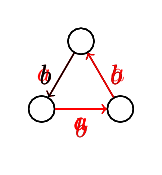
\begin{tikzpicture}
            \graphbox{\( \)}{0mm}{0mm}{20mm}{20mm}{-5mm}{-14mm}{
                \node[draw,circle] (x) at (0,0) {};
                \node[draw,circle] (y) at (1,0) {};
                \node[draw,circle] (z) at (0.5,0.86) {};
                \draw[->,red] (x) -- node[midway,below] {$a$} (y) ;
                \draw[->,red] (y) -- node[midway,right] {$b$} (z) ;
                \draw[->] (z) -- node[midway,left] {$b$} (x) ;
            } 
            \graphbox{\( \)}{22mm}{0mm}{20mm}{20mm}{-5mm}{-14mm}{
                \node[draw,circle] (x) at (0,0) {};  
                \node[draw,circle] (y) at (1,0) {};
                \node[draw,circle] (z) at (0.5,0.86) {};
                \draw[->] (x) -- node[midway,below] {$b$} (y) ;
                \draw[->,red] (y) -- node[midway,right] {$a$} (z) ;
                \draw[->,red] (z) -- node[midway,left] {$b$} (x) ;
            }
            \graphbox{\( \)}{44mm}{0mm}{20mm}{20mm}{-5mm}{-14mm}{
                \node[draw,circle] (x) at (0,0) {};   
                \node[draw,circle] (y) at (1,0) {};
                \node[draw,circle] (z) at (0.5,0.86) {};
                \draw[->,red] (x) -- node[midway,below] {$a$} (y) ;
                \draw[->,red] (y) -- node[midway,right] {$b$} (z) ;
                \draw[->] (z) -- node[midway,left] {$b$} (x) ;
            } 
            \graphbox{\( \)}{66mm}{0mm}{20mm}{20mm}{-5mm}{-14mm}{
                \node[draw,circle] (x) at (0,0) {};  
                \node[draw,circle] (y) at (1,0) {};
                \node[draw,circle] (z) at (0.5,0.86) {};
                \draw[->,red] (x) -- node[midway,below] {$b$} (y) ;
                \draw[->] (y) -- node[midway,right] {$b$} (z) ;
                \draw[->,red] (z) -- node[midway,left] {$a$} (x) ;
            }
            \graphbox{\( \)}{88mm}{0mm}{20mm}{20mm}{-5mm}{-14mm}{
                \node[draw,circle] (x) at (0,0) {};   
                \node[draw,circle] (y) at (1,0) {};
                \node[draw,circle] (z) at (0.5,0.86) {};
                \draw[->,red] (x) -- node[midway,below] {$a$} (y) ;
                \draw[->,red] (y) -- node[midway,right] {$b$} (z) ;
                \draw[->] (z) -- node[midway,left] {$b$} (x) ;
            }
         \end{tikzpicture}
         \caption{Sequence of rewriting steps, to be read left to right. In each graph, the subgraph to be replaced to obtain the next graph is highlighted in red.}
          \label{fig:intro:sequence_of_transformation_infinite}
        \end{figure}
Many termination techniques exist for term rewriting systems~\cite{nipkow1998term, dershowitz1982orderings, middeldorp1997simple, arts2000termination,contejean2005mechanically,urbain2004modular,contejean2011automated,giesl2014proving}.  
Most exploit the tree structure of terms, a feature absent in general graphs, making direct adaptation impossible. 
% Therefore, new techniques are needed for proving termination of DPO graph rewriting systems.  
Moreover, termination may not be the most pertinent property for our purposes. 

For example, consider the graph transformation system with two rules shown in Figure~\ref{fig:intro:edge_deletion_and_node_addition_rule}. Rule $\alpha$ deletes an arbitrary edge, and rule $\beta$ introduces a fresh node. The system does not terminate because the node-adding rule $\beta$ can be applied indefinitely. However, the edge-deleting rule $\alpha$ can be applied a finite number of times only: it deletes an edge on each application, and since no rule increases the edge count and the initial graph is finite, only finitely many deletions are possible. Therefore, termination of the full system depends solely on the node-adding rule $\beta$. This observation motivates the notion of \emph{relative termination}.

% \begin{center}
% in the following Figure~\ref{fig:intro:edge_deletion_and_node_addition_rule}
  \begin{figure}[H]
        \centering
%   \begin{subfigure}{0.3\textwidth}
%         % \centering
        $\alpha$ = {
             \resizebox{0.85\textwidth}{!}{
             \begin{tikzpicture}[baseline=-7ex]
                    \graphbox{\( \mathcal{L} \)}{0mm}{-3mm}{34mm}{15mm}{2mm}{2mm}{
                        \coordinate (o) at (0mm,-11mm); 
                        \node[draw,circle] (l1) at ($(o)+(-10mm,0mm)$) {$1$};
                        \node[draw,circle] (l2) at ($(l1)+(2,0)$) {$2$};
                        \draw[->] (l1) -- (l2) node[midway,above] {};
                    } 
            
                    \graphbox{\( \mathcal{K} \)}{40mm}{-3mm}{34mm}{15mm}{2mm}{2mm}{
                        \coordinate (o) at (0mm,-11mm); 
                        \node[draw,circle] (l1) at ($(o)+(-10mm,0mm)$) {$1$};
                        \node[draw,circle] (l2) at ($(l1)+(2,0)$) {$2$};
                    }  
            
                    \graphbox{\( \mathcal{R} \)}{80mm}{-3mm}{35mm}{15mm}{5mm}{2mm}{
                        \coordinate (o) at (-5mm,-11mm); 
                        \node[draw,circle] (l1) at ($(o)+(-10mm,0mm)$) {$1$};
                        \node[draw,circle] (l4) at ($(l1) + (2,0)$) {$2$};
                    }    
                    \node () at (37mm,-10mm) {\( \leftarrowtail \)}; % K -> L
                    \node () at (77mm,-10mm) {\( \rightarrowtail \)}; % K -> R
                \end{tikzpicture}
            }
        }
    %     \caption{A graph transformation rule for edge deletion}
    % \label{fig:intro:edge_deletion_rule}
    % \end{subfigure}
    
    % \begin{subfigure}{0.3\textwidth}
    %     % \centering

        $\beta$ ={
             \resizebox{0.85\textwidth}{!}{
             \begin{tikzpicture}[baseline=-7ex]
                    \graphbox{\( \mathcal{L} \)}{0mm}{-3mm}{34mm}{15mm}{2mm}{2mm}{
                        
                    } 
            
                    \graphbox{\( \mathcal{K} \)}{40mm}{-3mm}{34mm}{15mm}{2mm}{2mm}{
                       
                    }  
            
                    \graphbox{\( \mathcal{R} \)}{80mm}{-3mm}{35mm}{15mm}{5mm}{2mm}{
                        \coordinate (o) at (0mm,-11mm); 
                        \node[draw,circle] (l1) at ($(o)+(-10mm,0mm)$) {};
                    }    
                    \node () at (37mm,-10mm) {\( \leftarrowtail \)}; % K -> L
                    \node () at (77mm,-10mm) {\( \rightarrowtail \)}; % K -> R
                \end{tikzpicture}
            }
        }
    %     \caption{A graph transformation rule for node addition}
    %     \label{fig:intro:node_addition_rule}
    % \end{subfigure} 
    \caption{Rule $\alpha$ deletes an edge, and rule $\beta$ adds a fresh node.}
    \label{fig:intro:edge_deletion_and_node_addition_rule}
  \end{figure}
% \end{center}


\section{Relative termination} 
Relative termination was initially introduced for binary relations~\cite{klop1987term}: let $\mathcal{A}$ and $\mathcal{B}$ be two binary relations, $\mathcal{A}$ is said to be terminating relative to $\mathcal{B}$ if, for any infinite sequence of elements \( x_0, x_1, \ldots \) with \( (x_i,x_{i+1}) \in \mathcal{A} \) or \( (x_i,x_{i+1}) \in \mathcal{B} \) for all \( i \in \mathbb{N} \), there are only finitely many \( i \in \mathbb{N} \) such that \( (x_i,x_{i+1}) \in \mathcal{A} \).

Since a set of rewriting rules defines a binary relation \enquote{object $X$ can be rewritten to object $Y$ using rules from the rule set}, called a rewriting relation,
the concept of relative termination
carries over to rewriting systems in a straightforward way via their associated rewriting relations: a rule set $\mathcal{A}$ terminates relative to another rule set $\mathcal{B}$, if the binary relation induced by $\mathcal{A}$ terminates relative to the binary relation induced by $\mathcal{B}$.
% let \( \mathcal{A} \) and \( \mathcal{B} \) be two sets of rewriting rules, \( \mathcal{A} \) is said to be relatively terminating with respect to $\mathcal{B}$ if, for any infinite sequence of elements \( x_0, x_1, \ldots \) with $x_i$ can be rewritten to $x_{i+1}$ by a rule in $\mathcal{A}$ or $\mathcal{B}$ for all \( i \in \mathbb{N} \), there are only finitely many \( i \in \mathbb{N} \) such that $x_i$ can be rewritten to $x_{i+1}$ by a rule in $\mathcal{A}$. 
As an example, consider the edge-deleting rule $\alpha$ and the node-adding rule $\beta$, defined earlier and shown in Figure~\ref{fig:intro:edge_deletion_and_node_addition_rule}. 
The rule set $\set{\alpha}$ terminates relative to the rule set $\set{\beta}$, because any infinite sequence of graph transformations can apply the edge-deleting rule only finitely many times.

Relative termination generalizes termination in the context of rewriting, because a set of rules terminating relative to an empty set is terminating. In practice, to prove termination of a rewriting system $\mathcal{R}$, one partitions the set of rules into two disjoint subsets \( \mathcal{B} \) and \( \mathcal{A} \) with non-empty $\mathcal{A}$ such that \( \mathcal{A} \) terminates relative to \( \mathcal{B} \), if $\mathcal{B}$ is not empty then the termination of $\mathcal{R}$ is established, otherwise, a new iteration starts with the strictly smaller rule set $\mathcal{B}$.
 
Relative termination has several advantages.
  Firstly, by eliminating irrelevant rules, it lets us concentrate
  termination analysis on the essential part of the system.
  Secondly, it allows for different methods to be combined straightforwardly, leveraging each method's strengths, since different approaches can be tried at each iteration.
   Thirdly, when combined with Plump's modular termination technique~\cite{plump2018modular}\textemdash which proves termination by establishing the termination of two rule sets that partition the system's rule set\textemdash termination analysis becomes much easier.


\section{Termination of DPO graph rewriting systems on edge-labeled directed multigraphs} 
We consider DPO graph rewriting systems on edge-labeled directed multigraphs in this thesis, even though, using the language of category theory, it is possible to develop termination techniques for DPO rewriting systems on different graph notions that satisfy certain properties. There are several reasons for this choice. 

First of all, edge-labeled directed multigraphs are simple and intuitive: they are just directed graphs with multiple edges between two nodes allowed, and each edge is labeled by a symbol from a finite alphabet. This notion of graph is widely used in the literature, such as in the work introducing the DPO graph rewriting~\cite{ehrig1973graph}, in previous work on the method that we extend in Chapter~\ref{chap:nwf}~\cite{bruggink2014termination,bruggink2015proving,zantema2014termination}, and in illustrative examples of works~\cite{overbeek2024termination_lmcs,endrullis2024generalized_icgt} which are closely related to our work in Chapter~\ref{chap:subgraph_counting} and Chapter~\ref{chap:antipattern}.

 Secondly, by using this notion of graph, we want to avoid overly abstract reasoning and make the techniques more accessible to users than those based on more abstract notions of graphs, such as adhesive categories~\cite{lack2004adhesive}.
 As a consequence, the correctness of our technique in Chapter~\ref{chap:subgraph_counting} and Chapter~\ref{chap:antipattern} can be checked easily by users with basic knowledge in graph theory and very basic knowledge in category theory.

Finally, specializing to edge-labeled directed multigraphs enables us to leverage graph-specific properties to develop stronger termination criteria. Because termination is undecidable for general DPO graph rewriting systems~\cite{plump1998terminationundecidable}, this specialization is essential for extending the boundaries of practically verifiable termination. 

% Chapter~\ref{chap:nwf} extends a existing method for termination of DPO graph rewriting systems, called type graph method~\cite{zantema2014termination,bruggink2014termination,bruggink2015proving,endrullis2024generalized_icgt}. This work resulted in the following publication:
% \begin{itemize}
% \item Qi Qiu. Termination of Graph Rewriting using Weighted Type Graphs over Non-well-founded Semirings. 16th International Workshop on Graph Computation Models, Jun 2025, Koblenz, Germany. 2025. ⟨hal-04954960v3⟩
% \end{itemize}
 
%  Chapter~\ref{chap:subgraph_counting} introduces a new machine-checkable sufficient condition for relative termination of DPO graph rewriting with injective rules on edge-labeled multigraphs. The method is based on counting injective graph homomorphisms: let $\mathcal{A}$ and $\mathcal{B}$ be two sets of rewriting rules, if the number of injective homomorphisms from a chosen set of pattern graphs into the host graph strictly decreases when a rule from $\mathcal{A}$ is applied, and the number does not increase when any rule from $\mathcal{B}$ is applied, then rules in $\mathcal{A}$ can only be applied finitely many times.
% This work resulted in the following publication:
% \begin{itemize}
%     \item Qiu, Q. (2025). Termination of Injective DPO Graph Rewriting Systems Using Subgraph Counting. In: Endrullis, J., Tichy, M. (eds) Graph Transformation. ICGT 2025. Lecture Notes in Computer Science, vol 15720. Springer, Cham. \url{https://doi.org/10.1007/978-3-031-94706-3_1}
% \end{itemize}

%  Chapter~\ref{chap:antipattern} extends the technique introduced in Chapter~\ref{chap:subgraph_counting} to handle cases like the one shown in Figure~\ref{fig:intro:{fig:intro:graph_transformation_rule_anti_pattern_}} which cannot be addressed by the method presented in Chapter~\ref{chap:subgraph_counting}.
 
%  Chapter~\ref{chap:lyonparallel} presents a termination tool, \textit{LyonParallel}, developed for DPO edge-labeled multigraph rewriting that integrates the existing type graph method, our extension presented in Chapter~\ref{chap:nwf}, and our technique presented in Chapter~\ref{chap:subgraph_counting} and its extension presented in Chapter~\ref{chap:antipattern}.
\section{Contributions}
% \paragraph{Contribution 1: Extension of Weighted Type Graph Method}\ \newline
Chapter~\ref{chap:nwf} extends a existing method for termination of DPO graph rewriting systems, called type graph method~\cite{zantema2014termination,bruggink2014termination,bruggink2015proving,endrullis2024generalized_icgt}. 
The method assigns weights to morphisms targeting a weighted type graph over a well-founded semiring. The weight of a graph is defined
 as the sum of the weights of all morphisms from that graph to the type graph. Relative termination of $\mathcal{A}$ with respect to $\mathcal{B}$ is proven by ensuring that rewriting steps using rules in \( \mathcal{A} \) strictly decrease the weights of the host graphs, while rewriting steps using rules in \( \mathcal{B} \) do not increase them. However, searching for a suitable type graph over a well-founded semiring is challenging. We propose to consider type graphs over non-well-founded semirings, which can be easier to find in some scenarios. 
% \paragraph{Contribution 2: Termination by Morphism Counting}
% \ \newline

Chapter~\ref{chap:subgraph_counting} introduces a new automated technique for relative termination of DPO graph rewriting with injective rules on edge-labeled multigraphs.
The method is based on counting injective graph homomorphisms: let $\mathcal{A}$ and $\mathcal{B}$ be two sets of rewriting rules, if the number of injective homomorphisms from a chosen set of pattern graphs into the host graph strictly decreases when a rule from $\mathcal{A}$ is applied, and the number does not increase when any rule from $\mathcal{B}$ is applied, then rules in $\mathcal{A}$ can only be applied finitely many times. This technique can handle some cases that prior interpretation-based approaches cannot.
Proofs of all propositions, lemmas, and theorems of this chapter
 have been moved to Appendix~\ref{subgraph_counting:sec:appendix} to improve readability.
% \begin{itemize}
%     \item Qiu, Q. (2025). Termination of Injective DPO Graph Rewriting Systems Using Subgraph Counting. In: Endrullis, J., Tichy, M. (eds) Graph Transformation. ICGT 2025. Lecture Notes in Computer Science, vol 15720. Springer, Cham. \url{https://doi.org/10.1007/978-3-031-94706-3_1}
% \end{itemize}

% \paragraph{Contribution 3: Termination by Morphism Counting with Antipattern}
% \ \newline
Chapter~\ref{chap:antipattern} extends the technique introduced in Chapter~\ref{chap:subgraph_counting} to handle rewriting systems with rules like the following one:
%  shown in Figure~\ref{fig:intro:graph_transformation_rule_anti_pattern__}.

% \begin{figure}[H]
%     \centering
\begin{center}
    \resizebox{0.85\textwidth}{!}{
\begin{tikzpicture}
      \graphbox{$\mathcal{L}$}{0mm}{0mm}{34mm}{20mm}{2mm}{-5mm}{
          \coordinate (o) at (0mm,-3mm); 
          \node[draw,circle] (l1) at ($(o)+(-10mm,0mm)$) {$1$};
          \node[draw,circle] (l2) at ($(l1)+(2,0)$) {$2$};
          \node[draw,circle] (l3) at ($(l1) + (1,0)$) {$3$};
          \draw[->] (l1) -- (l3) node[midway,above] {$a$};
          \draw[->] (l3) -- (l2) node[midway,above] {$a$};
      }     
      \graphbox{$\mathcal{K}$}{40mm}{0mm}{24mm}{20mm}{2mm}{-5mm}{
          \coordinate (o) at (5mm,-3mm); 
          \node[draw,circle] (l1) at ($(o)+(-10mm,0mm)$) {$1$}; 
          \node[draw,circle] (l2) at ($(l1)+(1,0)$) {$2$};
      }    
      \graphbox{$\mathcal{R}$}{70mm}{0mm}{45mm}{20mm}{2mm}{-5mm}{
        \coordinate (o) at (0mm,-3mm); 
        \node[draw,circle] (l1) at ($(o)+(-10mm,0mm)$) {$1$};
        \node[draw,circle] (l2) at ($(l1)+(2,0)$) {$2$};
        \node[draw,circle] (l3) at ($(l1) + (1,0)$) {$3$};
        \draw[->] (l1) -- (l3) node[midway,above] {$a$};
        \draw[->] (l3) -- (l2) node[midway,above] {$a$};
        \draw[->] (l3) edge [loop below] node {$c$} (l3);
      }    

      \node () at (37mm,-10mm) {$\leftarrowtail$};
      \node () at (67mm,-10mm) {$\rightarrowtail$};
  \end{tikzpicture}
    }
\end{center}
%   \caption{}
%   \label{fig:intro:graph_transformation_rule_anti_pattern__}
%  \end{figure} 
In this example, the number of injective graph homomorphisms from every pattern graph increases with each application of the rewriting rule. Therefore, the method introduced in Chapter~\ref{chap:subgraph_counting} cannot be applied. However, if we restrict our attention to occurrences of pattern graphs that are not part of a larger occurrence of a specific graph, the number of such occurrences decreases with each application of the rewriting rule. 
Proofs of all propositions, lemmas, and theorems of this chapter have been moved to Appendix~\ref{antipattern:sec:appendix} to improve readability.

A purely theoretical contribution to automated reasoning would make little sense if it did not lead to a software tool that implements it.

Chapter~\ref{chap:lyonparallel} introduces the termination tool \textbf{LyonParallel} for DPO edge-labeled multigraph rewriting, which integrates the existing type graph method, our extension, and our morphism counting technique and its extension.  